\documentclass[tikz,border=8pt]{standalone}

\usepackage{mathpazo}        
\usepackage{amsmath}      
\usepackage{tikz}
\usetikzlibrary{positioning,arrows.meta,calc, shapes}

\definecolor{petrol}{RGB}{34,139,34}
\definecolor{pet}{RGB}{0,222,225}

\newlength{\bw}\setlength{\bw}{2.4cm}
\newlength{\bh}\setlength{\bh}{0.95cm}
\tikzset{
  comp/.style  ={draw,rounded rectangle,fill=petrol!18,
                 minimum width=\bw,minimum height=\bh,align=center},
  projC/.style ={draw,rectangle,fill=green!15,
                 minimum width=\bw,minimum height=\bh,align=center},
  projS/.style ={draw,rectangle,fill=orange!18,
                 minimum width=\bw,minimum height=\bh,align=center},
  cloud/.style ={draw,rectangle,fill=cyan!12,
                 minimum width=\bw,minimum height=\bh,align=center},
  otbox/.style ={draw,rectangle,fill=cyan!28,
                 minimum width=\bw,minimum height=\bh,align=center},
  merge/.style ={draw,rectangle,fill=gray!10,
                 minimum width=\bw,minimum height=\bh,align=center},
  loss/.style  ={draw,diamond,fill=red!10,aspect=2,
                 text width=1.45cm,align=center,inner sep=1pt},
  gate/.style  ={draw,circle,fill=yellow!20,minimum size=0.85cm},
  ntext/.style ={font=\small\scshape},           
  line/.style  ={->,>=Latex,line width=0.55pt}
}

\tikzset{
  exp/.style={
    draw            = blue!60!black,   
    fill            = pet!8,        
    rounded corners = 6pt,
    text width      = 3cm,
    inner xsep      = 9pt,
    inner ysep      = 9pt,
    font            = \small,
    align           = center
  }
}

\begin{document}
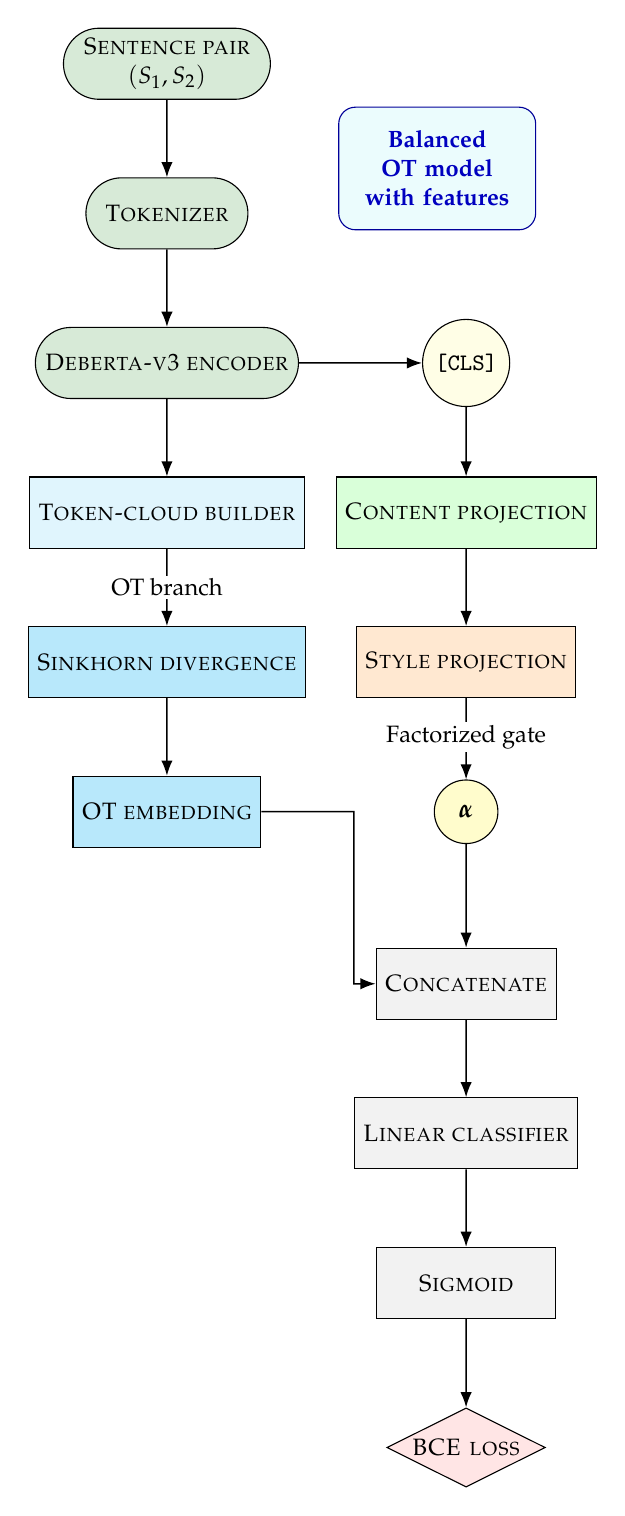
\begin{tikzpicture}[scale=0.95,transform shape]


\node[comp,ntext] (inp)   {Sentence pair\\$(S_1,S_2)$};
\node[comp,ntext] (tok)   at ($(inp)+(0,-2.0)$)  {Tokenizer};
\node[comp,ntext] (enc)   at ($(tok)+(0,-2.0)$)  {Deberta-v3 encoder};

\node[cloud,ntext] (cloud) at ($(enc)+(0,-2.0)$)  {Token-cloud builder};
\node[otbox,ntext] (sink)  at ($(cloud)+(0,-2.0)$){Sinkhorn divergence};
\node[otbox,ntext] (otemb) at ($(sink)+(0,-2.0)$) {OT embedding};


\def\colX{4.0}                       
\node[circle,draw,fill=yellow!10,font=\small]
      (cls)  at (\colX,-4.0) {\texttt{[CLS]}};

\node[projC,ntext] (cont) at ($(cls)+(0,-2.0)$) {Content projection};
\node[projS,ntext] (sty)  at ($(cont)+(0,-2.0)$){Style projection};

\node[gate,font=\normalsize] (mix)  at ($(sty)+(0,-2.0)$) {$\boldsymbol{\alpha}$};
\node[merge,ntext] (cat)  at ($(mix)+(0,-2.3)$){Concatenate};
\node[merge,ntext] (lin)  at ($(cat)+(0,-2.0)$){Linear classifier};
\node[merge,ntext] (sig)  at ($(lin)+(0,-2.0)$){Sigmoid};
\node[loss,font=\small\scshape] (bce) at ($(sig)+(0,-2.2)$){BCE loss};


\draw[line] (inp)  -- (tok);
\draw[line] (tok)  -- (enc);

\draw[line] (enc)  -- (cloud);
\draw[line] (cloud) -- (sink);
\draw[line] (sink) -- (otemb);


\draw[line] (enc) -- ($(enc)!0.5!(cls)$) -- (cls);
\draw[line] (cls)  -- (cont);
\draw[line] (cont) -- (sty);
\draw[line] (sty)  -- (mix);


\coordinate (aux) at ($(otemb)+(2.5,0)$);
\draw[line] (otemb) -- (aux) |- (cat);

\draw[line] (mix)  -- (cat);
\draw[line] (cat)  -- (lin);
\draw[line] (lin)  -- (sig);
\draw[line] (sig)  -- (bce);


\node[font=\small,fill=white,inner sep=1pt] at ($(mix)+(0,1.0)$) {Factorized gate};
\node[font=\small,fill=white,inner sep=1pt] at ($(sink)+(0,1.0)$) {OT branch};

\node[exp,                                
      text width=2cm,anchor=west,            
      right=1.2cm of tok.east,%              
      yshift=0.6cm]                              
      (bal)
{%
  \textbf{\small\textcolor{blue!75!black}{Balanced OT model\\with features}}%
};

\end{tikzpicture}
\end{document}